\documentclass{article}
\usepackage[utf8]{inputenc}
\usepackage[margin=1in]{geometry}
\usepackage{graphicx}
\usepackage{subfig}
\usepackage{url}

\setlength{\parskip}{1em}

\title{Fuzzy Clustering Library}
\date{13.5.2016}
\author{Eléonore d'Agostino et Benoît Zuckschwerdt}

\begin{document}
  \pagenumbering{arabic}
  \maketitle
  \tableofcontents
  \newpage

  \section{Introduction}

    Notre projet consiste à l'implémentation d'une variété d'algorithmes de Fuzzy Clustering dans l'idée d'en faire un ensemble de méthodes efficaces et facile d'usage.

  \section{Contexte}

    Le \textit{Clustering} consiste à prendre un ensemble de données, et à le diviser en groupes, ou \textit{clusters}.

    \subsection{Fuzzy Clustering}

      Aussi connu sous le nom de \textit{Soft Clustering}, le Fuzzy Clustering, à la différence du \textit{Hard Clustering}, permet à un point d'appartenir à zero où plusieurs clusters, et d'avoir un degré d'appartenance à chacun des clusters du système.

    \subsection{Algorithme K-means}

      Algorithme de hard clustering, K-means est l'algorithme de clustering le plus basique. Il génère des fonctions d'appartenance binaires, ne permettant que des valeurs de 1 (appartient au cluster) ou 0 (n'appartient pas au cluster).

      Le concept derrière K-means est de partitionner un ensemble d'observations $(x_1,x_2,...,x_n)$ de manière à minimiser le \textbf{WCSS}, où \textit{Within-Cluster Sum of Squares} (Somme des carrés interne au cluster), dont la formule est $\sum_{i=1}^{k}\sum_{x\in S_i}||x-\mu_i||^2$, où $\mu_i$ est la moyenne des points dans chaque cluster.

      L'algorithme standard de K-means, aussi connu sous le nom d'\textit{Algorithme de Lloyd}, fonctionne en alternant entre deux étapes, avec $c_1^{(1)},...,c_k^{(t)}$ l'ensemble initial de $k$ centres:

      L'étape \textbf{d'assignement} lie chaque observation $x_p$ au cluster dont le centre donne le WCSS minimal. Ceci correspond à partitionner les observations suivant le diagramme de Voronoi généré par les centres: chaque $x_p$ est assigné à un et un seul cluster $S^{(t)}$, avec $S_i^{(t)}=\{x_p:||x_p-c_i^{(t)}||^2\leq ||x_p-c_j^{(t)}||^2\forall j,1\leq j\leq k\}$

      L'étape de \textbf{mise à jour} calcule des nouveaux centres correspondant au centres géométriques des nouveaux clusters, en minimisant le WCSS. On a alors $m_i^{(t+1)}=\frac{1}{|S_i^{(t)}|}\sum_{x_j\in S_i^{(t)}}x_j$

      Dès qu'on atteint une itération où l'étape de mise à jour ne modifie plus de valeurs, l'algorithme se termine.

      Par contre, l'algorithme K-means doit être initialisé avec deux informations: le nombre de clusters désirés, ainsi que les moyennes initiales pour chacun de ses clusters. Dans le cas le plus simple, les moyennes initiales sont obtenues au hasard parmis les observations déjà présentes.

      \newpage
      \subsubsection{K-means++}

        K-means++ propose une solution au problème d'initialisation de l'algorithme K-means. Un problème majeur avec prendre les moyennes initiales de manière aléatoire est que les clusters résultant seront potentiellement différents à chaque lancement de l'algorithme. L'idée de K-means++ est de tenter de trouver des moyennes initiales éloignées des autres, sans pour autant commencer sur des observations aberrantes.

        L'algorithme de K-means++ fonctionne aussi de manière iterative. On commence par choisir un "centre" uniformément aléatoirement parmi les observations, puis on alterne entre deux étapes jusqu'à avoir choisi les $k$ points voulus:

        \begin{enumerate}
          \item Pour chaque point $x$, on calcule $D(x)$, la distance entre $x$ et le centre le plus proche.
          \item On choisi un nouveau centre aléatoirement, mais pas de manière uniforme. On utilise une distribution où chaque point $x$ est choisi avec une probabilité proportionelle à $D(x)^2$.
        \end{enumerate}

        Ceci prend plus de temps que d'initialiser K-means de manière complètement aléatoire, mais le K-means après est plus efficace et tournera en moyenne moins longtemps pour un meilleur résultat.

    \subsection{Algorithme Fuzzy C-means}

      Le concept de C-means est similaire à celui de K-means, mais en logique floue plutôt qu'en logique binaire. La principale différence est que plutôt que de calculer l'appartenance à un cluster comme étant $\{0,1\}$ avec une appartenance à un seul cluster par point, on calcule les coefficients d'appartenance à chaque cluster pour chaque observation, pour avoir $[0,1]$ d'appartenance par cluster, avec un total de 1.

      Ceci veut dire que plutôt que d'avoir un ensemble de clusters $S$, on travaille avec une matrice $W=w_{i,j}\in [0,1], i=1,...,n, j=1,...,c$ où chaque élément $w_{i,j}$ correspond au degré auquel l'observation $x_i$ appartient au cluster $c_j$, et le WCSS correspond à $\sum_{i=1}^n\sum_{j=1}^c w_{ij}^m ||x_i-c_j||^2$, où $w_{ij} = \frac{1}{\sum_{k=1}^c (\frac{||x_i-c_j||}{||x_i-c_k||}) ^{\frac{2}{m-1}}}$.

      $m \geq 1$ est le \textit{fuzzifier}, qui détermine le niveau de flou des clusters. Plus $m$ est élevé plus les degrés d'appartenance seront bas, et inversément. La valeur la plus commune est $m=2$, et $m=1$ donne des résultats presque identiques à K-means.

      Additionellement, comme C-means travaille avec des valeurs réelles là où K-means utilise des valeurs binaires, l'algorithme prend fin lorsque que le changement des coefficients entre deux itérations est inférieur à $\varepsilon$, le seuil de sensibilité donné.

    \subsection{Algorithmes Expectation-Maximization}

      L'Expectation-Maximization (où \textit{EM}) est une catégorie d'algorithmes travaillant de manière itérative avec deux étapes principales. La partie \textbf{Expectation} qui calcule des espérances, et la partie \textbf{Maximization} qui cherche quel paramètre peut maximiser cette quantité.

      L'algorithme K-means est un exemple d'application d'un algorithme EM, mais il est possible de prendre directement un EM comme source pour ensuite tenter de génerer des clusters de manière différente que le K-means. En particulier, en appliquant des filtres ou en utilisant des algorithmes de réduction de bruit à l'étape d'expectation. Les filtres de Kalman (où estimation linéaire quadratique) sont particulièrement utiles dans les cas où les observations pourraient contenir du bruit.

  \section{Etat de l'art}

  Les fonctions que nous allons mettre en place sont utilisées dans des domaines variés, par exemple pour:
  \begin{itemize}
    \item la météorologie
    \item l'analyse d'images
    \item le marketing
    \item la bioinformatique
    \item la biologie
    \item la médecine
    \item ou encore la psychologie
  \end{itemize}

  Il existe encore beaucoup d'autres domaines concernés, on constate que l'utilité de ces fonctions est immense.


  Nous passons ici en revue quelques outils possédant des implémentations de ces même fonctions.

  \subsection{SciPy}

  SciPy est une librairie Python possédant une implémentation de K-means.

  \subsection{Scikit}

  Scikit est une autre librairie Python, mais cette fois possédant une implémentation de K-means et C-means.

  \subsection{Mathematica}

  Mathematica est un logiciel de calcul édité par Wolfram Research. Il possède une implémentation de C-means.

  \subsection{MATLAB}

  MATLAB est un language de programmation, il est utilisé à des fins de calculs numériques.

  Ce langage possède une implémentation de C-means,
  mais également une implémentation de Subtractive Clustering
  qui est un algorithme pour estimer le nombres de clusters pour un jeu de données.

  %Fuzzy C-Means Clustering et Subtractive Clustering -> http://ch.mathworks.com/help/fuzzy/fuzzy-clustering.html?requestedDomain=www.mathworks.com

  \subsection{R}

  R est un logiciel libre de traitement de données et d'analyse statistique, il utilise le langage de programmation S.
  Il possède trois variantes de K-means et une fonction nommée FANNY similaire à C-means mais offrant la possibilité d'utiliser une
  une matrice nXn symmétrique qui mesure a quel point deux objets sont différents.

  %FANNY -> https://stat.ethz.ch/R-manual/R-devel/library/cluster/html/fanny.html
  % ET: http://www.r-bloggers.com/fuzzy-clustering-with-fanny/

  \section{Réalisation}

  Nous allons développer nos fonctions en Python, ce choix nous semble le plus logique, vu qu'on utilise ce language dans ce cours.

  Pour commencer nous allons mettre en place K-means dont l'implémentation est plus simple que celle de C-means,
  cela nous permettra également de bien comprendre le fonctionnement des ces méthodes et par la suite de les comparer (C-means étant de la logique floue).

  Nous nous intéresserons ensuite aux algorithmes Expectation-Maximization avec divers filtres, ainsi qu'à des algorithmes permettant de calculer le nombres de cluster plutôt que de demander une entrée manuelle (tel \texttt{Subtractive clustering} de Matlab).

  \section{Implémentation}

  Nous avons implémenter en Python K-means, K-means++ (pour les centres) et C-means.

  \subsection{K-means}

  L'implémentation de K-means nous a permis de bien comprendre et aborder le sujet.
  Son implémentation s'est avéré largement plus facile que celle de C-means.

  \subsection{K-means++}

  Nous avons implémenté K-means++ et nous l'utilisons avec K-means et C-means pour déterminer les centres.
  Avant d'utiliser cette algorithme, nous choisissions manuellement les centres.
  K-means++ nous permis d'avoir de bien meilleures résultats.


  \subsection{C-means}

  L'implémentation de C-means c'est avéré plus difficile que celle de K-means,
  nous avons passé beaucoup de temps dessus pour que cela fonctionne bien et
  par conséquent nous avons préféré avoir une bonne implémentation fonctionnelle
  de C-means au lieu d'avoir un C-means et un EM qui ne fonctionnent pas.

  Pour mettre en place C-means, nous avons chercher plusieurs documents, et
  à notre grande surprise les formules données étaient souvent un peu différentes.
  Finalement, nous nous sommes surtout basé sur le document suivant:\\
  \url{https://sites.google.com/site/dataclusteringalgorithms/fuzzy-c-means-clustering-algorithm}


  \section{Résultats}

  Notre implémentation possède un mode \texttt{verbose} permettant d'afficher beaucoup
  d'informations supplémentaires, c'est très utile pour le debug et également pour mieux comprendre ce qui est fait.

  \subsection{Iris Dataset}

  Nous avons choisi d'utiliser le Iris Dataset comme exemple, pour plusieurs raisons;
  nous avons déjà travaillé dessus et ce dataset est très connu ce qui nous a permis de
  pouvoir comparer nos résultats avec d'autres sur le Web.

  \begin{figure}[h]
    \centering
    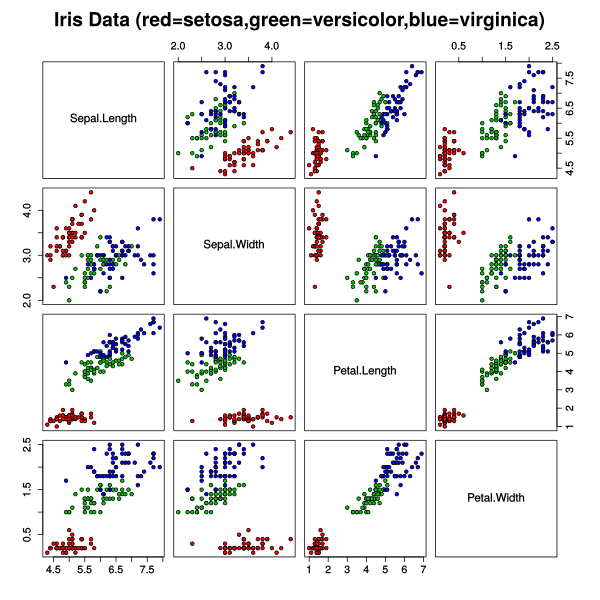
\includegraphics[scale=0.5]{images/Iris_dataset_scatterplot.png}
    \caption{Scatterplot du dataset (source: wikipedia.org)}
    \label{fig:scatterplot-wiki}
  \end{figure}

  Vu que l'Iris Dataset possède 4 attributs (sepal length, sepal width, petal length, petal width),
  nous ne pouvons pas représenter le tout sur un seul plot 3D, nous avons donc choisi de prendre les trois premiers attributs
  pour représenter les axes
  et d'utiliser la couleur des points pour représenter les clusters.

  Source du dataset: \url{archive.ics.uci.edu/ml/datasets/Iris}

  \newpage
  Les différents couleurs représentent les clusters, les trois variétés d'iris (Setosa, Versicolour et Virginica) (figure \ref{fig:kmeans-iris}).

  Sur la figure \ref{fig:kmeans-iris} on peut voir les erreurs en rouge.

  \begin{figure}[h]
    \centering
    \subfloat{{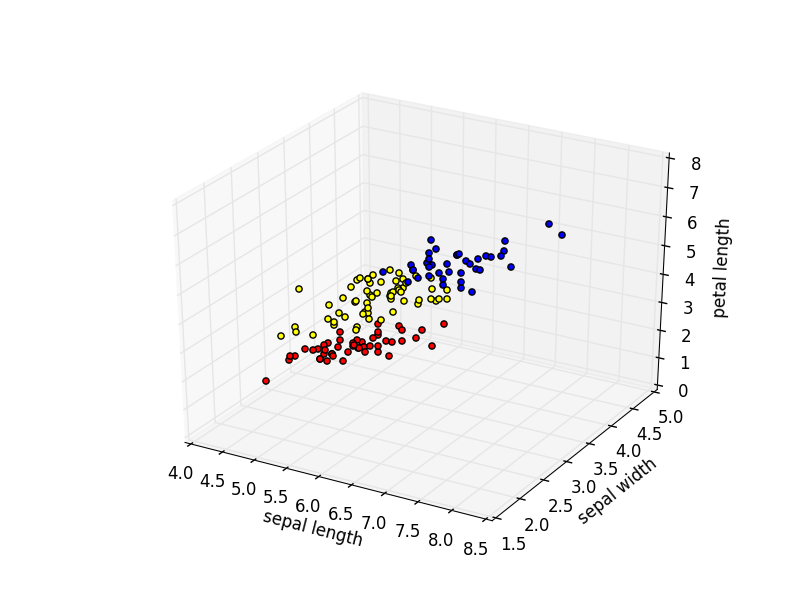
\includegraphics[width=0.45\textwidth]{images/kmean-cluster.png}}}%
    \qquad
    \subfloat{{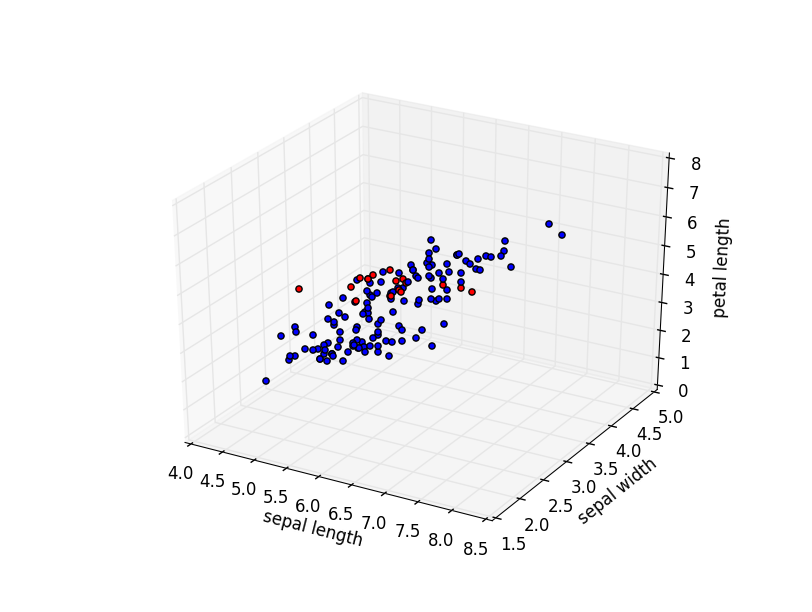
\includegraphics[width=0.45\textwidth]{images/kmean-false.png}}}%
    \caption{K-means: (gauche) plot 3D, (droite) erreurs en rouge}%
    \label{fig:kmeans-iris}
  \end{figure}

  \subsection{Traitement d'images}

  Comme second exemple nous avons décidé de travailler sur des images, puisqu'il s'agit de l'exemple le plus parlant que nous avons pu trouver. En effet, même quelqu'un n'étant pas dans le domaine peut facilement voir et comprendre le résultat obtenu.

  Nous nous sommes limités à des petites images (la plus grande a des dimensions de 50x50 pixels), vu que les temps de calculs avec 16 clusters atteignaient les minutes.

  Les images sont présentées avec l'image originale tout à gauche, suivi des résultats de K-means en haut, et les résultats de C-means en bas, chacun montrant le résultat à 2, 4, 8, et 16 clusters respectivement.

  \begin{figure}[h]
    \centering
    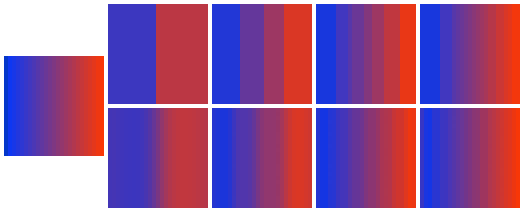
\includegraphics[width=\textwidth]{images/concat_testing_mini.png}
  \end{figure}

  Ce premier exemple utilise un simple dégradé, et on remarque qu'avec suffisamment de clusters, on voit de moins en moins de différences entre les résultats.

  \begin{figure}[h]
    \centering
    
\includegraphics[width=\textwidth]{images/concat_boss.png}
  \end{figure}

  \newpage
  Ce deuxième exemple est affiché avec du noir pour symboliser la transparence, montrant que le script fonctionne même avec des informations d'alpha. On remarque que C-means permet de perdre beaucoup moins de détails, même avec très peu de clusters, mais a tendance à avoir des centres de clusters moins distincts que K-means.

  \begin{figure}[h]
    \centering
    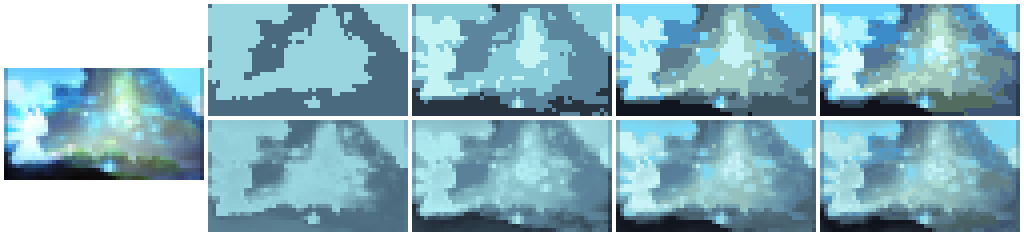
\includegraphics[width=\textwidth]{images/concat_test.png}
  \end{figure}

  Ce dernier exemple emploie plus de couleurs et est moins \textit{discret} que les deux précédentes. Similairement aux autres exemples, C-means donne de bien meilleurs résultats si on se limite à 2 ou 4 clusters, mais obtients des centres moins intéressant que K-means quand on augmente les clusters.

  \newpage
  \section{Utilisation}
    \subsection{Fonctions internes}

    \subsection{Interactions avec Iris}

    \subsection{Interaction avec images}

  \section{Conclusion}

  Ce projet nous a permis de bien comprendre K-means et C-means, le fait de devoir les implémenter
  manuellement nous a pousser à connaître ces algorithmes de manières très détaillés.
  Nous avons malheureusement pas pu implémenter l'algorithme Expectation-Maximization,
  ceci à cause des difficultés rencontrées lors de l'implémentation de C-means.
  Il nous a paru mieux d'arriver à avoir une bonne implémentation fonctionnelle de C-means,
  au lieu d'avoir deux algorithmes non fonctionnnelles.
  Concernant l'application de ces algorithmes,
  il a était très intéressant de pouvoir les appliquer sur le Iris Dataset, mais également sur les images.

\end{document}
